\glsresetall

\chapter{Related Work}
This review of related past work focuses on the three main areas of Computer Science that are relevant to this dissertation:  Stereo Matching, Formal Models of Computation (especially \gls{ps}), and \glsentrylong{cml-glossary}.  In none of these cases does the review come close to comprehensively covering the entire span of the given area.  It merely tries to cover as much of the relevant recent and classic work as possible, while giving an extremely brief introduction to these areas.  The interested reader who is unfamiliar with any of these topics is strongly advised to refer to the materials cited.

\section{Formal Models of Concurrent Computation}
Perhaps the earliest (or at least, the earliest that is still widely known) formalised model of concurrent computation is the Petri Net \cite{Dennis2011}, first conceived of by Carl Petri, initially for the purpose of describing chemical processes \cite{Petri2008}.

\begin{anfxerror}{Why not Petri Nets?}
Why are Petri Nets not more popular?  Why do we choose \gls{csp} or \glspl{actor} or \gls{ps} over them?
\end{anfxerror}

\cite{Varela2013}

This work 

\subsection{\glsentrylong{csp} \& Pi~Calculus}
\gls{csp} is a `process algebra' and abstract model of concurrent computation put forward by Hoare \cite{Hoare1985,Roscoe2011}.  A typical sequential computation is represented by a `process'.  Processes' ``behaviour is described in terms of the occurrence and availability of abstract entities called \textit{events}'' \cite[p.~478]{Roscoe2011}.  Should more than one event be available simultaneously for a given process, then one will be chosen non-deterministically.  This choice is internal to the process, and not influenced by or visible to any other process.  %E.g. for a situation where there is one possible event \(a\) at a given point in time, the process \(P\) will choose that event and then proceed according to the result, written as: \[ a \rightarrow P(a) \]

Concurrency is introduced by the existence of multiple processes.  In general, the processes evolve independently, responding to events as they come.  Should a particular event appear in the alphabet of multiple processes, however, then all processes \emph{must} choose to participate in that event at the same time.  Should all processes involved make such a choice, they engage in a synchronous multi-way atomic synchronisation (hence `communicating').  \gls{csp} has provided significant inspiration for concurrency design in a number of programming languages, notably including Ada \cite{Defense1983,Taft2013}, Occam \cite{Elizabeth1987}, Google's Go \cite{Meyerson2014} (not to be confused with the earlier language Go! \cite{Clark2004}, which itself was explicitly designed for concurrency) and \gls{cml} \cite{Reppy2011}. 

Milner appreciated \gls{csp}, which advanced concurrency models by explicitly incorporating \emph{synchronised} interaction, something Milner's earlier Calculus for Communicating Systems \cite{Milner1980} had lacked  \cite{Milner1993}.  Milner still regarded \gls{csp} as incomplete, however, in that it had no support for the concept of `mobility' -- i.e. the ability of the system to reconfigure itself during operation.  Pi Calculus was created as an attempt to build upon those earlier systems but present a complete calculus of concurrent computation in much the same way that Lambda Calculus \cite{Barendregt1984} is a complete calculus for sequential computation.\footnote{Milner also pointed out that sequential computation is, in fact, a special case of concurrent computation.}

\subsection{\label{subsec:actors}\texorpdfstring{\Glspl{actor}}{Actors}}
The \gls{actor} \cite{Agha1986} model was introduced by Hewitt \cite{Hewitt1973}.  Much like \gls{csp} \& its cousins, the \gls{actor} model is based around the concept of separated, sequential but communicating processes which exchange messages.  Again, the processes make decisions and proceed based on their communications.  A key difference, however, is that in the \gls{actor} model the message exchanges are \emph{a}synchronous.  Each \gls{actor} has its own `mailbox', and may send messages to other \glspl{actor} so long as it knows their name (which is equivalent for this purpose to a concept of an address for the \gls{actor}), \emph{but does not wait at all for a response before proceeding}.

The \gls{actor} model is a popular one for concurrent programming, possibly owing to its intuitive concept.  The fact that communication is asynchronous makes \glspl{actor} much more suitable for modelling distributed systems without shared memory than \gls{csp} or similar -- \glspl{actor} can send messages and proceed without (necessarily) needing to wait for a response, instead continuing to process based on the messages they themselves have received.  By contrast, a system with synchronous communication would have prohibitive time costs, given the relative slow speed of typical links between distributed computers as compared to their capacity for local processing.  Many \gls{actor} systems have been implemented for different programming languages (e.g. \cite{Varela2001,Srinivasan2008,Charousset2016,Bernstein2016} \fxnote[inline,nomargin]{[need more refs?]}), and in fact it is a core component, and perhaps largely responsible for the success, of Erlang/OTP \cite{Armstrong2010,Armstrong2013,Vinoski2012}.  A relatively new language, Pony \cite{Clebsch2015,Clebsch2017}, takes this even further.
\begin{anfxnote}{Positive example for actors?}
In Concurrency in .NET, Terrell described using an actor to control access to a shared resource and stated that it was an extremely effective solution.
\end{anfxnote}

\Glspl{actor}, when used for non-trivial real-world software, have been criticised at times \cite{Welsh2013,Stucchio2013}.  While some of the criticisms described are implementation-specific (relating to Akka, a Scala \gls{actor} library), a common thread is that \glspl{actor} do not compose well.  This has the negative consequence that it is difficult to combine an \gls{actor} with anything else to create a new abstraction, and can require extensive modifications in source code to make relatively simple changes.

\subsection{Join Calculus}

\begin{anfxwarning}{Join Calc refs}
Chemical abstract machine, joinads, Scala communicating objects (IIRC, that was join calculus based), reagents
\end{anfxwarning}

\subsection{Others}
Mobility calculus.  Others?

% \subsection{Criticisms}

% Gorlatch \cite{Gorlatch2004} argued against basic message passing, decrying it as an unnecessary and unhelpful complication and favouring \fxerror*{What does `collective operations' mean?}{`collective' operations} instead.  This criticism focused upon \gls{mpi} as it was at the time, however, and made no reference to either Actors or \gls{csp}. \fxerror{Does subsection this truly belong here?}

\section{\glsentrytext{ps}/\glsentrytext{mc}}
\gls{ps}, also known as \gls{mc} (the two terms are generally used interchangeably), is a bio-inspired model of computing created by Păun in the late 1990s \cite{tPaun98a,Paun2000}, originally conceived of by considering the process of chemical reactions and exchanges that occur inside living biological cells \& the membranes within, and regarding this process as a form of computation.

Păun describes \gls{mc} \cite[p.~VII]{Paun2002} as:
\begin{quote}
Membrane computing is a branch of natural computing which abstracts from
the structure and the functioning of living cells. In the basic model, the membrane
systems - also called P systems - are distributed parallel computing
devices, processing multisets of objects, synchronously, in the compartments
delimited by a membrane structure. The objects, which correspond to chemicals
evolving in the compartments of a cell, can also pass through membranes.
The membranes form a hierarchical structure - they can be dissolved, divided,
created, and their permeability can be modified. A sequence of transitions between
configurations of a system forms a computation. The result of a halting
computation is the number of objects present at the end of the computation
in a specified membrane, called the output membrane. The objects can also
have a structure of their own that can be described by strings over a given
alphabet of basic molecules - then the result of a computation is a set of
strings.
\end{quote}

\Gls{mc} works analogously to a typical modern electronic computer, in that the system stores data, and processes \& updates those data based on a predefined program, with a view to arriving at a computable answer based on the starting state and any inputs to the system \cite{Paun2002,Paun2010b}.  In the case of \gls{ps}, the data are multisets of symbols, representing various chemicals and their quantities.  These are found inside one or more cells, based on real biological cells, which (to a certain extent at least) form a hybrid between main memory and the processing units of a computer.  The instructions of the program itself are provided by rules, which specify transformations of objects and interactions with the surrounding environment and other membranes or cells.

There are now, broadly, three main families of \gls{ps} variants:  \gls{clps} \cite{Paun2001,Paun2002}, \gls{tlps} \cite{tMaPaPaRo01a,Martin-Vide2003} and \gls{snps} \cite{Ionescu2006}.\footnote{Several other variants have been created, but most are used infrequently, if ever.  Apart from Numerical \gls{ps} and \gls{cps}, described in \autoref{subsec:numpsys} and \autoref{subsec:cpsys} respectively, this work will not address them.}  \Gls{clps} is the original, and sees objects compartmented into `membranes', which are arranged in a graphical tree structure with the outermost membrane (separating the cell from its environment) as the root of the tree.  In most variants, objects can evolve inside a membrane, but also be communicated between membranes (and the environment).  Furthermore, membranes can divide or dissolve themselves, and may have one or more special properties, such as `polarization' \cite{Paun1999a}.

Conversely, \gls{tlps} and \gls{snps} both arrange their computing compartments, named `cells' or `neurons' respectively, as nodes in arbitrary digraphs, with the edges between them representing connecting channels.  Whereas \gls{clps} emphasise the evolution of multisets of objects inside compartments, \gls{tlps} and \gls{snps} emphasise communication between separate cells/neurons, and many \gls{tlps} variants do not include any capacity for internal evolution inside cells -- if new objects are required, they are imported via communication with the environment, which is considered to possess an unlimited number of all objects, but has no rules of its own.

While \gls{tlps} have arbitrary alphabets, only one object is used in \gls{snps}, the `spike'.  This means that \gls{tlps} are frequently much like \gls{clps} in that they have custom objects for each purpose, with the key difference (usually) being in how the \glspl{prox} are arranged relative to each other and the choice between the two motivated primarily by which one seems like a better fit to the computation to be modelled.

Conversely, \gls{snps} represent everything through the use of differing quantities of the spike, kept in different neurons.  This means that it can be more complex to model certain problems, but also arguably means that \gls{snps} are, \textit{prima facie}, closer to Lambda Calculus \cite{Barendregt1984} and Church Numerals \fxerror[inline]{[ref]}, as well as Register Machines \fxerror[inline]{[ref]} (and indeed Register Machines have been simulated with \gls{snps} \fxerror[inline]{[ref]}).  All three approaches have been proven Turing-universal though \fxerror[inline]{[ref]}, so all three should be capable of expressing the same computations in different forms.  Furthermore, because \gls{snps} can easily be represented numerically, they lend themselves well to vector/matrix representations \cite{Zeng2010}.  This means that, potentially, \gls{snps} implementations can take advantage of high-performance techniques such as using \gls{blas} and/or \glspl{gpu} \cite{Aboy2019}.

Arguably, the most notable and important aspects of \gls{ps} models are that they:  i) Generally have no space limit.  That is, they contain an arbitrary number of cells, objects and membranes;  ii) Across all cells and membranes, all rules that can be applied are applied, as many times as possible given the current number of objects available.  These two features mean that \gls{ps} have unbounded space and processing capacity, which can be used to solve traditionally computationally-difficult problems relatively quickly \cite{Sosik2003,Jimenez2003,Paun1999a,Henderson2020}.  Most of these solutions, however, rely on trading time complexity for space complexity.  While this works in the theoretical framework, electronic simulations of the systems do not have access to unlimited instantaneous memory space, meaning many of the fast solutions are impractical with current real-world computers, e.g. \cite{Cooper2019} \fxnote[inline]{[refs]}.

\Gls{mc} is not just a theoretical model with limited practical use, however.  Besides Image Processing \& Computer Vision (see \autoref{subsec:imgprocpsys}), \gls{ps} variants have been applied to a range of fields, from power grid management to robotic control systems \cite{Zhang2017}.  [P-Lingua and simulation systems, e.g. MeCoSim]

\subsection{\label{subsec:numpsys}Numerical \glsentrytext{ps}}
Numerical P systemsss

\subsection{\label{subsec:cpsys}\glsentrytext{cps}}
\cite{Nicolescu2014b,Nicolescu2017}

\gls{cps} is another variant of \gls{ps}, developed by Nicolescu and collaborators in the early 2010s \fxerror[inline]{[ref]}.  It is largely based on \gls{clps}, and can be seen, to some extent at least, as a higher-level abstraction over it \cite{Nicolescu2018}.  It can also incorporate elements of \gls{tlps}, however, in that it includes concepts of channels and message passing between cells \cite{Henderson2019}.  Nicolescu, Ipate \& Wu demonstrated that not only is \gls{cps} capable of performing the same tasks as other \gls{ps} variants, but also can be used fairly cleanly to model typical computer programs \cite{Nicolescu2014a}.

The major advantage of \gls{cps} over traditional \gls{clps} is a simplification in the specification of complete systems to solve a given problem.  \gls{clps} (as well as \gls{tlps} and \gls{snps}) typically require the definition of a family of rulesets customised to the specific instance of the problem at hand, whereas \gls{cps} usually requires only the definition of a fixed (usually much shorter) set of rules that cover all possible instances.  Only inputs to the system need vary to solve different instances of the problem, e.g. in \cite{Cooper2019} only five fixed rules were needed to solve any instance of the Travelling Salesman Problem, with only customisation of the input objects (in this case, elements describing the nodes and edges of the graph) required.



\subsection{\label{subsec:imgprocpsys}Image Processing and Computer Vision in P~systems}
\cite{Zhang2012}

Perhaps owing to the unbounded potential space and parallelism of \gls{ps}, combined with the embarrassingly parallel nature of many tasks in Image Processing \& Computer Vision, the latter has proved to be fertile ground for the former, although not every publication puts its model to the test with a computerised simulation, or if it does, the authors may only provide scant details \cite{Diaz-Pernil2019}.  

Christinal, Díaz-Pernil \& Real \cite{Christinal2011} described a family of \gls{tlps} to perform region-based segmentation of both 2D and 3D images.  Despite their family of systems requiring only two cells, it also needed custom rule sets based on the size of the images as well as the number of colours present, with a number of rules per set proportional to the same measurements.  The paper showed the results of simulating the system, but provides no details on performance.

Díaz-Pernil \textit{et al.} \cite{Diaz-Pernil2013} commented that ``... commonly [a] parallel algorithm needs to be re-designed with only slight references to the [sequential original].  ... the design of a new parallel implementation not inspired by the sequential one allows ... the proposal of new creative solutions.''  They then demonstrated this fact by designing a new edge detection and segmentation algorithm named `A Graphical P (AGP) segmentator', inspired by the Sobel operator (see e.g. \cite{Nixon2012}) and using the segmentation method from \cite{Christinal2011}, which they modelled in \gls{tlps}.  The authors implemented their new algorithm on a \gls{gpu} and compared it with an implementation of the 3x3 and 5x5 Sobel operators, finding that theirs had near-identical runtimes but superior edge detection capabilities.

Díaz-Pernil \textit{et al.} \cite{Diaz-Pernil2013a} further explored modelling classic image processing techniques by implementing Guo \& Hall's binary image skeletonisation technique \cite{Guo1989} with \gls{snps}.  The overall system's rules templates are reasonably simple, but include references to a set \(DEL\) (used as a lookup to determine whether a cell should turn white or stay black) which does not appear to be modelled inside the system, meaning that it is not self-contained.  The authors simulated this system on a \gls{gpu}, but found that their implementation was upwards of twice as slow as another pre-existing implementation.  Confusingly, however, they state that one of the reasons for this is ``that the use of an alphabet with only one object, the spike \(a\), does not fit in the GPU architecture''.  This statement is difficult to understand, given that spikes can easily be represented as simple integers.  The authors also commented that the synchronous nature of the model is unrealistic, and imposing a global clock upon the system can be problematic.

Nicolescu \cite{Nicolescu2014} alternatively applied \gls{cps} to image skeletonisation based on Guo \& Hall's technique \cite{Guo1989}, presenting three forms of a solution: Synchronous versions that use multiple or a single cell (essentially the latter replicates the former via the use of sub-membranes), and an asynchronous multi-cell version.  The asynchronous version no longer assumes that all messages are passed between cells simultaneously and instantaneously, compensating for this by increasing the number of messages used.  This form, while arguably more realistic to modern computers, requires a greater message complexity. A prospective \gls{actor}-model-based (see \autoref{subsec:actors}) simplified implementation using \fsharp{}'s \texttt{MailboxProcessor} \cite[ch.~11]{Syme2015a} was presented also, but no results from running it were reported.

Nicolescu \cite{Nicolescu2015a} further applied \gls{cps} to seeded region growing of grayscale images.  The described system used a two-level approach, based on the `Structured Grid Dwarf' of the 13 Berkeley Dwarves \cite{Asanovic2006}, where the image was divided into rectangular blocks of multiple pixels.  Each block was modelled with a single cell, inter-block processing was carried out via message passing, and intra-block processing was performed by typical object evolution.  It was again suggested that this would fit well to the \gls{actor} model.

Díaz-Pernil \textit{et al.} \cite{Diaz-Pernil2016} built upon their AGP segmentator algorithm to create a version that works with RGB images rather than grayscale and applied it to a common medical Computer Vision task, isolating the `optic disc' in images of the inner eye.  With this they used the skeletonisation algorithm from \cite{Diaz-Pernil2013a} and a number of other steps not based on \gls{ps} to produce a complete imaging pipeline.  The authors implemented this on a \gls{gpu}, and found that their system was both more accurate and faster than previous systems.

Most directly relevant to the current work are \cite{GimelFarb2013a,Gimelfarb2011,Nicolescu2014b}, which model Dynamic Programming \gls{sm} in \gls{ps}, and indeed saw the genesis of \gls{cp} (\autoref{subsec:concprop}).  

\subsubsection{\glsentrytext{ps} on \glsentrylongpl{gpu}}
In many instances, a \gls{ps} model for a problem involves many separate small elements processing their data separately, and perhaps updating each other's state at the end of a step.  Given that this sounds remarkably close to the Single-Instruction Multiple-Thread \cite[Ch. 4.4.1]{Hennessy2012} nature of modern \gls{gpgpu}, it is no surprise that there has been much work put into simulating \gls{ps} on \glspl{gpu}.

\cite{Cecilia2010,Cecilia2010a,Cecilia2013,Macias-Ramos2015,Martinez-Del-Amor2015,Martinez-Del-Amor2013a,Maroosi2014,Maroosi2014a}


\section{\glsentrylong{mpbsm}}

% \subsection{Preliminaries}
% What do I actually need to put in here?

% \subsubsection{Stereo Matching}

\subsection{\label{subsec:smgeneral}\glsentrytext{sm} in General}
Szeliski defines \gls{sm} \cite[p. 469]{Szeliski2011} as ``the process of taking two or more images and estimating a 3D model of the scene by finding matching pixels in the images and converting their 2D positions into 3D depths.''  It is essentially an attempt to replicate one of the techniques the brain uses to provide depth perception,\footnote{The brain has others, such as exploiting familiarity with everyday objects to estimate their actual size, and thus their rough distance from the eyes.} namely correlating the images received from each eye to estimate the distances to objects within view, but using digital images and a computer.

Indeed, \gls{sm} is not the only method for computer depth perception in use \cite{Sinha2020}.  Other approaches include, for example, Structured Light \cite{Giancola2018}, Time-of-Flight \cite{Hansard2013} and LiDAR \cite{Dong2017}.  \Gls{sm} has some advantages over those other techniques, though.  It is the only one which is entirely passive, i.e. it takes in data from the environment without interacting with it in some way, whereas the other three all involve projecting some form of light into the environment.  It is also arguably quicker to perform the necessary observations of the environment than the other methods, in that only a single pair of images need be captured, which can be accomplished in the time it takes for the pixel values to be read from the sensor planes into storage.  The choice of which method is most appropriate depends heavily upon the intended use of the computerised depth perception.  Or, if sufficient processing power is available, two or more of them can be used in combination to offset each other's weaknesses \cite{Zanuttigh2016}.

The `canonical' stereo camera arrangement is two cameras arranged in parallel, with a small horizontal offset between them.  This configuration leads to a general expectation that changes in the points in the scene will be shifted along one image's x-axis as compared to the other image's.  The identified distance of a shift is termed the `\gls{disparity}', and is used with other information about the cameras to compute an estimate to the matched points in the scene.  Generally, it is \fxnote*{name of assumption?}{assumed} that points in the image from the left camera will appear further to the right in said image as compared the same point in the right camera's image, and vice versa.

\begin{figure}
    \centering
    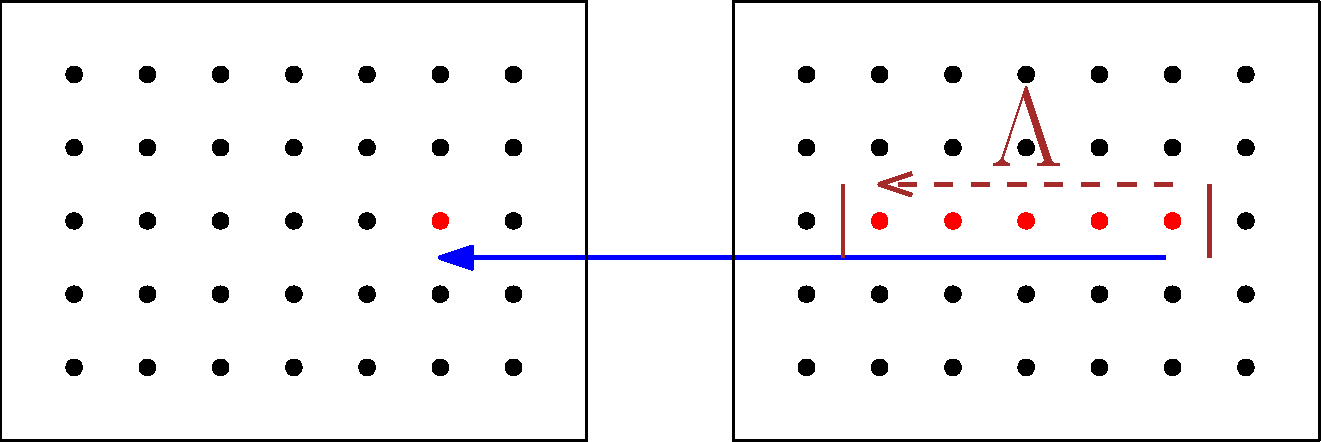
\includegraphics[width=1.0\textwidth]{chapters/litreview/images/stereo_matching-eps-converted-to.pdf}
    \caption{Diagram of the basic process of \gls{sm}. In this instance, for each pixel in the left image, a horizontal range of the pixels in the right image are searched, to find the one on the right that matches most closely to the one on the left. This has the effect that the \gls{disparitymap} is from the perspective of the left camera. The red dots represent the compared pixels. The brown dashed arrow and vertical bars represent the range of pixels in the right image to compute matching scores against. The length of the range is the lesser of the number of pixels before reaching the left border of the image, or the maximum \gls{disparity}, which is a parameter set by the user and represented here by \(\Lambda\).  Image from \cite{bsmpcvpic}.}
    \label{fig:stereomatchingbasic}
\end{figure}

% While precise approaches vary, the vast majority of \gls{sm} algorithms utilise some form of pixelwise comparison between images.  The basic process for this is shown in \autoref{fig:stereomatchingbasic}.    This comparison function be as simple as taking the absolute difference of the pixels under comparison.

In the general case \gls{sm} is impossible to perform perfectly because it is an ill-posed problem \cite{Gimelfarb1998}.  Going from a three-dimensional scene to a two-dimensional image necessarily involves a loss of information.  For any given image there are potentially an unbounded number of possible real-world scenes that could produce said image.  Using multiple images -- the more the better -- for \gls{sm} permits some recovery of information, but the process inevitably suffers from various sources of noise (where `noise' is defined broadly).

Liu \textit{et al.} \cite{Liu2005} describe four types of noise:  Signal, geometric, electronic and optical.  Signal noise arises from the normal operation of digital cameras, and electronic from differences between the internal operation of cameras used to capture images from different perspectives of the same scene.  Optical noise mainly stems from differences in the intensity and colour of light seen by the cameras at different perspectives when capturing images of the scene, caused by differences in the interactions between the objects of the scene and the available light sources at different points.  Lastly, geometric noise is a natural consequence of the fact that different perspectives must be used, and can be caused by issues as simple as the fact that points visible in one scene may not be visible in the other -- so-called `occlusions', caused by one part of the scene obscuring another part.

A key consequence of the last source of noise is the fact that, even in ideal circumstances with multiple `perfect' cameras, flawless lighting throughout the scene and \fxnote*{Provide reference for Lambertian surfaces}{objects which do not reflect light differently at different parts of their surfaces}, occlusions mean that for an arbitrary scene it is impossible to be certain a given algorithm has achieved a perfect reconstruction of the depths of the scene \cite{Gimelfarb1998}.  Strictly speaking, it \emph{is} possible that \gls{sm} produces an entirely accurate \gls{disparitymap}, but there would be no way to know without the use of additional information.

\fxwarning[inline,nomargin]{Include some example images to show the idea of stereo matching?}

\subsubsection{Image Rectification}
To reduce the computational complexity involved in performing \gls{sm}, many, perhaps most, algorithms only directly compare pixels along a single line in each image, typically the same horizontal line \cite[Ch. 11]{Szeliski2011}.  If the lines in the two images do not correspond to roughly the same part of the scene, then the matching process will likely fare poorly.  Such a discordance can occur when the cameras were not adequately aligned in terms of their spatial positions and angles relative to each other at the time of mutual image capture.

To overcome the challenges caused by mismatched lines, stereo image pairs are usually `rectified' (see e.g. \cite[Ch. 1.5.1]{Wohler2013}), wherein the captured images are adjusted so that they were effectively \fxerror*{Rectification could be described more precisely}{taken by properly aligned cameras}.  If rectification is performed well, the lines in the image should be properly aligned.  The parameters used in rectification in turn are deduced via camera calibration (see e.g. \cite[Ch. 1.4]{Wohler2013}), though neither topic is discussed further here.  For current purposes, all stereo image sets used are assumed to have been appropriately rectified already.

\begin{anfxnote}{}
    Discuss epipolar geometry?
\end{anfxnote}

\subsubsection{Middlebury}
\fxnote[inline,nomargin]{Talk about the Middlebury benchmarks, resources and website here.}

\subsubsection{Local vs Global}
\fxerror*{Expand/explain}{\cite{Scharstein2002}  (similar terms were in use earlier \cite{Gimelfarb1998})}

Perhaps the simplest and most obvious ways to perform \gls{sm} involve simply comparing the values of pixels in one image to the values of pixels in the other.

\subsubsection{\glsentrylong{mrf} \& Bayesian Inference}
\fxerror*{Expand/explain}{\cite{Kolmogorov2015,Blake2011}}

Not all global \gls{sm} algorithms utilise message passing, e.g. Graph Cuts \cite{Kolmogorov2001,Tappen2003}

Geman \& Geman \cite{Geman1984} showed that \glspl{mrf} are equivalent to Gibbs Distributions and that the two could be applied usefully to image tasks \cite{Gimelfarb1999}.

\begin{anfxwarning}{Pixel similarity measures}
    Move the below discussion about pixel similarity measures further up, probably into the \gls{sm} in general section?
\end{anfxwarning}

Frequently, in global methods the function used for the data cost is quite simplistic.  Most common is the use of simple absolute difference between the intensities of the pixels compared.  Other popular methods include \gls{sad} and \gls{ssd} \fxerror[inline]{[ref]}, adaptive window methods \cite{Yoon2005,Yoon2006}, and Birchfield \& Tomasi's Pixel Dissimilarity Measure \cite{Birchfield1998}.

In general, most \gls{mrf} approaches to \gls{sm} tend to use a truncated linear function to estimate the discontinuity/smoothness cost.  Such a function typically takes a form such as \[ E_{discontinuity} = \alpha \times min(| d_p - d_q |, \beta) \] where, for the purposes of this equation, \(E_{discontinuity}\) represents the total estimated cost of the assignment; \(\alpha\) is a scaling coefficient that may or may not be used; \(\beta\) is a constant that provides the upper limit to the cost estimate; and \(d_p\) and \(d_q\) are the proposed \fxwarning*{labels?}{labels} of the current pixel and its neighbour currently under consideration.  While a simple absolute difference function is perhaps the most common applied to the labels, it is important to note that it is not the only one that could be used.  

For example, Ha and Jeong \cite{Ha2016} use a two-step \fxnote*{Define Potts model}{Potts model}, with different penalties for a difference of 1 compared to a difference of 2 or greater. Conversely, Tan \textit{et al.} \cite{Tan2017} comment that a typical Potts function can be viewed as a special case of the absolute difference truncated linear function, where the truncation value (\(\beta\) in the equation above) is 1, while the coefficient is the value of the Potts penalty parameter.

The choice of the truncated linear function is motivated by the assumption that most surfaces in images either are planar, or smoothly vary in disparities, and thus larger jumps should be penalised more heavily, but very large jumps are almost certainly indicative of an object boundary where a large difference in disparities is warranted.  Therefore, at a certain point, the penalty to assign significantly different values should stop growing, so as not to reduce the likelihood of correctly assigning large differences in disparities at object edges.

\subsection{Dynamic~Programming}

\gls{dpsm} was first introduced by Gimel'farb, Marchenko and Rybak in 1972 \cite{Gimelfarb1972}.\footnote{There is a popular misconception that \gls{dpsm} was introduced in the 1980s with \cite{Ohta1985}.  This is plainly false, given that \gls{dpsm} was first described years earlier.  The confusion is unsurprising, however, because \cite{Ohta1985} was likely the first description of \gls{dpsm} many in the English-speaking world saw, as a consequence of the Cold War.  For example, the authors \cite{Salmen2009} of seem to have this misunderstanding.}  

% \begin{anfxnote}{DP's streaking}
%     Be sure to mention the streaking commonly seen with \gls{dpsm} -- if nothing else it will be important for explaining why \gls{sgm} was created.
% \end{anfxnote}

Anecdotally, variants of \gls{dpsm} are still popular in practical applications of \gls{sm} because it tends to give acceptable results \fxerror[inline]{[ref?]} and is amenable to fast implementations with low-powered devices \fxerror[inline]{[ref?]}.

\begin{anfxnote}{Why mention DP?}
    Partly because it is a basis for other algorithms, but at least as much because the process of propagating information up and down the scanlines that it entials is very much reflective of message passing.  ``The main difference between DP and 1D BP is the word `message' '' -- Georgy (at my provisional).  Something similar was mentioned in appendix B to \cite{Szeliski2011}.
\end{anfxnote}

\subsubsection{Symmetric Dynamic Programming Stereo}
Motivated by observations of the physical reality of the image capture process and propounded by Gimel'farb \fxerror*{Expand/explain}{\cite{Gimelfarb1979,Gimelfarb2001} + \cite{Nguyen2013,VanMeerbergen2001}.  \cite{Khan2016}}

\subsection{\glsentrylong{bp}}
\gls{bp} was introduced by Pearl \cite{Pearl1982} for use with inference engines, in the context of Bayesian Statistics \fxerror[inline]{[ref]} and Gibbs Distributions \fxerror[inline]{[ref]}.  \gls{bp} was first applied to \gls{sm} in \cite{Sun2003} where it demonstrated excellent matching performance compared to many contemporary matching algorithms, but the `breakthrough' paper was arguably \cite{Felzenszwalb2006}, where a near-real time implementation was presented which still had extremely good results.  Szeliski commented in c. 2011 that \gls{lbp} was still used at that time in some of the best-performing \gls{sm} algorithms \cite[p. 163]{Szeliski2011}.

\begin{figure}
    \centering
    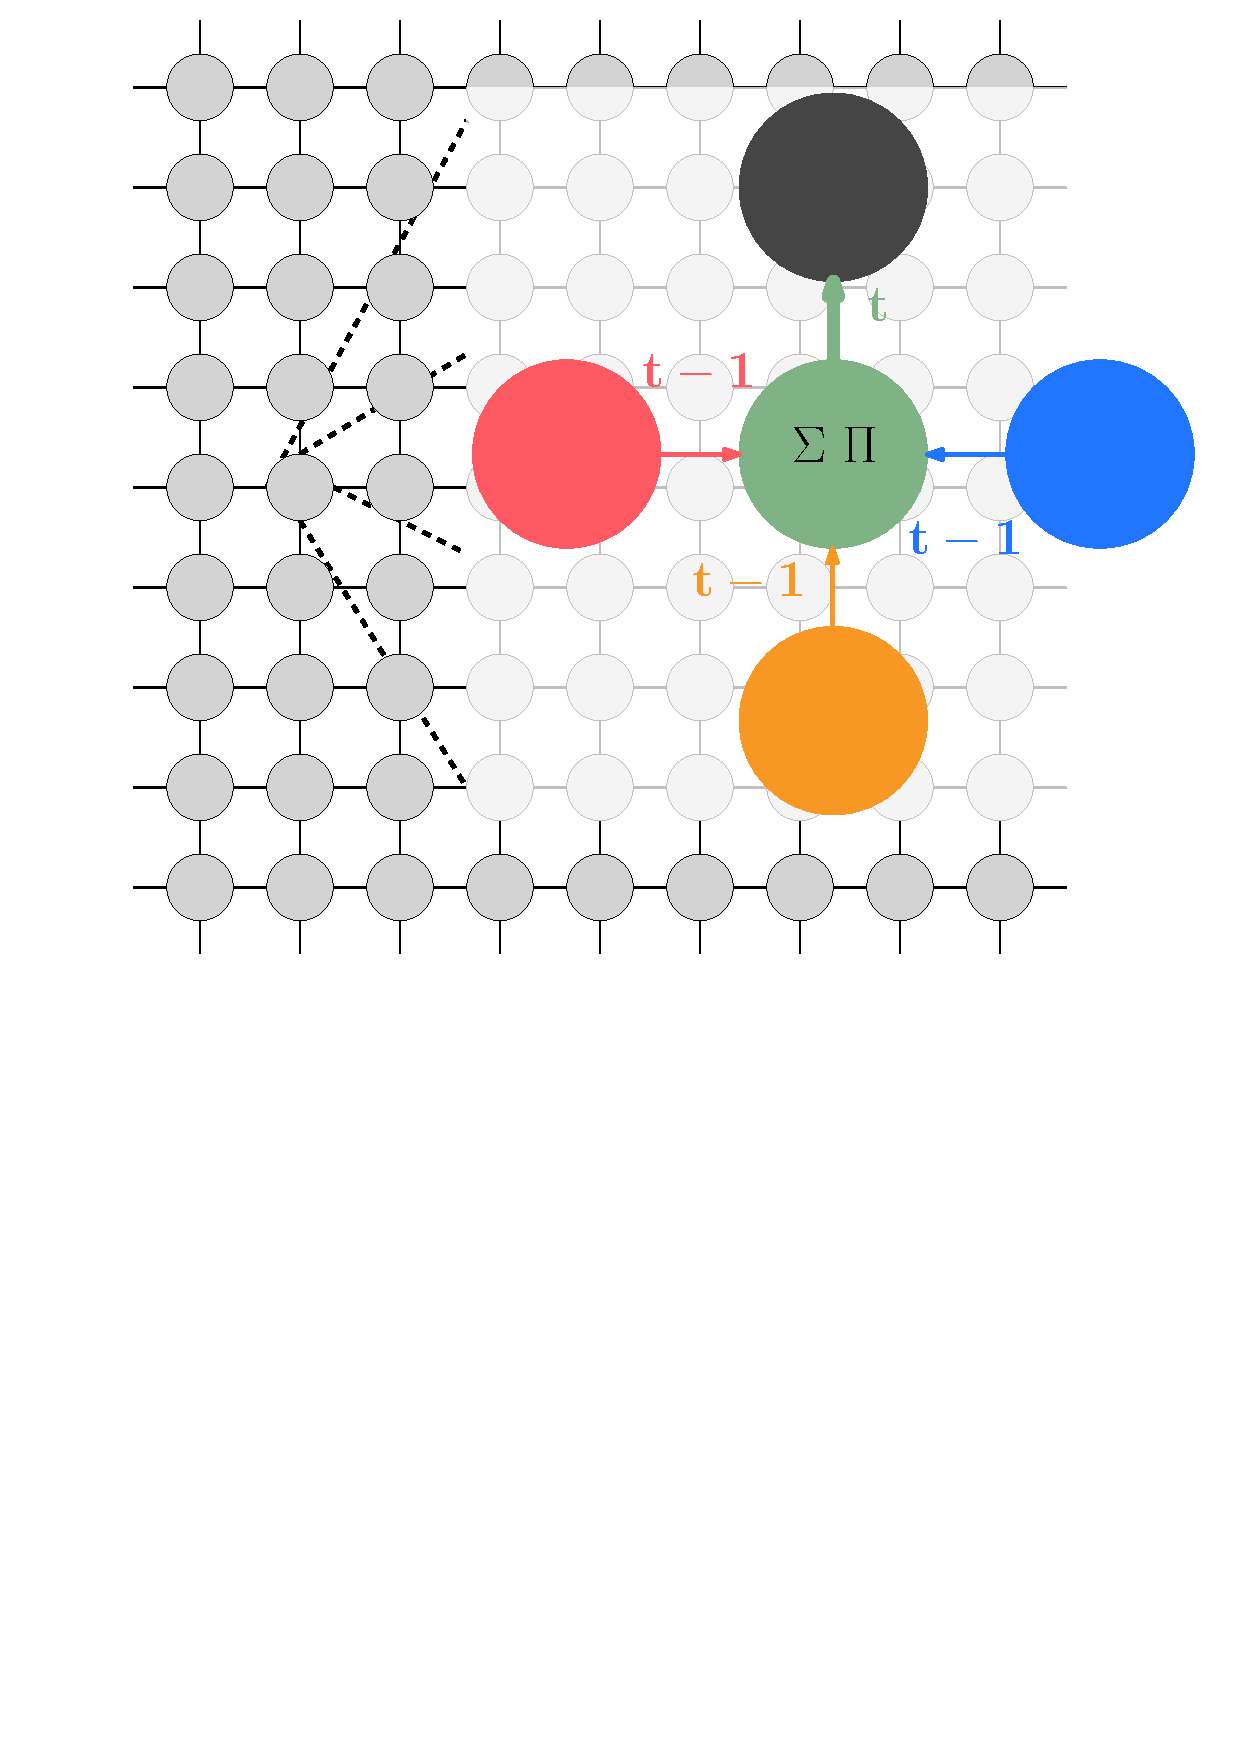
\includegraphics[width=1.0\textwidth]{chapters/litreview/images/bp_diagram_recoloured.pdf}
    \caption{Pictorial representation of the concept behind Loopy Belief Propagation for Stereo Matching. The symbols in the central cell refer to sum-product Belief Propagation, one of the earliest and mostly widely discussed forms of Belief Propagation. Each cell sends a new message to its neighbouring cells at each iteration after in turn having received and processed new messages from the neighbours in the previous iteration. The outgoing message to a given neighbour is computed from the information received from the other neighbours previously, represented here by the three thin and one fat arrow.  Image from \cite{lbpmpsmpic}.}
    \label{fig:bpdiagram}
\end{figure}

Yang \textit{et al.} \cite{Yang2006a} built upon \fxerror*{Explain hierarchical BP}{hierarchical \gls{bp}}, adding in extra steps before and after the \gls{bp} process.  They combine information derived from using the mean shift algorithm \cite{Comaniciu2002}; a colour-weighted correlation method based on Yoon \& Kweon's \cite{Yoon2006} applied to both the left and right images; a left-right consistency check to detect occluded pixels; a plane-fitting process based on Tao \& Sawhney's \cite{Tao2000}; as well as \gls{bp} itself.  While combining these various techniques leads to a highly-accurate disparity map,\footnote{This algorithm achieved the top ranking on Middlebury when it was first introduced.} this approach is \emph{extremely} slow.

Typical \gls{bp} uses the four-connected neighbourhood to define the neighbours of each given node in the grid.  This means that each node passes messages to and from it's immediate neighbours up, down and to the left and right of it in the grid.  Other neighbourhood arrangements are possible though, depending on the underlying model one wants to use.  For example, Tan \textit{et al.} \cite{Tan2017} describe an approach to \gls{bp} where every pixel is considered to be a neighbour of every other pixel.  Messages are weighted according to the distance across the grid between the neighbours, with nearer neighbours having a greater impact upon a pixel's final beliefs.  The major advantage of this approach is that it almost eliminates the need for repeated iterations of message passing.

Ha and Jeong \cite{Ha2016} suggested a different approach for scheduling the messages.  Instead of each pixel repeatedly exchanging messages with its neighbours until a reasonable amount of the grid has been spanned, they start in one of the corners in the image, and sequentially pass messages along two directions until reaching the other corner, repeating this process once for each corner.  The great advantage of this is that in principle one only needs to perform message exchanges in each direction once.  Their implementation still required roughly \SI{3.5}{\second} to complete, however, without returning a significantly more accurate disparity map.\footnote{The authors claimed that their method was \numrange{300}{600} times faster than `standard` \gls{bp}, but they did not specify their stopping condition.  Based on their reported results it appears that they used well over 300 iterations on an image with their standard comparison -- many more than would be reasonable for image sizes likely to be targeted for real-time \gls{sm}.}

Balossino \textit{et al.} \cite{Balossino2007} suggested an alternative formulation to the traditional grid of \gls{lbp}.  Instead, they built a forest of trees, each of which was rooted at the given pixel under consideration, and which has a handful of neighbouring pixels as children.  The attraction of this approach is that it restores the properties of optimality and convergence described in \cite{Pearl1982} for one round of messages up and down each tree.  This advantage is tempered, however, by the necessity of combining results from different trees.  The final accuracy appeared to be worse than with \cite{Felzenszwalb2006}, and there was no reporting of the running time, though it seems unlikely that this approach was fast.

It should be noted that \gls{bp} is \emph{not} regarded as the current top-performing \gls{sm} algorithm.  Tippets \textit{et al.} found c. 2012 that, of algorithms implemented on the CPU, SADL from \cite{VanDerMark2006} was the fastest accurate-enough method, and ADCensus from \cite{Mei2011} was the most accurate, and in fact was described as ``Pareto-optimal'' by Tippets \textit{et al.}  \fxnote{Move this paragraph?}  In terms of \gls{gpu} implementations, the algorithm from \cite{Zhao2011} was the fastest by far (though it only properly worked when observing scenes with motion).  The authors do not state an overall most-accurate \gls{gpu}-based algorithm, but based on Fig. 7 in \cite{Tippetts2016}, it appears that the \gls{gpu} implementation of the ADCensus algorithm from \cite{Mei2011} was again the best.\footnote{Other, faster, algorithms were also discussed, but those required specialist hardware such as \glspl{fpga} or \glspl{dsp}.}  \Gls{bp} \emph{is} amenable to parallelisation (unlike its traditional rival, Graph Cuts \cite{Tappen2003}) and \gls{gpu} implementations, but the main point of interest for it in this work is the fact that it is explicitly built around the concept of independent processing elements exchanging messages.

\begin{anfxwarning}{Top algos on Middlebury}
    Thinking about it, I probably should investigate the current top-performing algorithms on Middlebury, at least the ones which have accompanying publications.
\end{anfxwarning}

\subsubsection{Real-time/resource-constrained \glsentrylong{bp}}
One of the major drawbacks of \gls{bp} as compared to a number of other approaches to \gls{sm} is that a simple naïve implementation is both quite slow, and very memory-intensive.  Slow because of the requirement to perform many iterations, and memory-intensive because \emph{at least} one copy of the data costs and the message estimates for each neighbour must be stored in memory, with the result that a number of values on the order of at least \(O(5XYD)\) are kept in memory, where X and Y are the width and height of the stereo images, and D is the size of the disparity range.

Seeking to derive the comparative benefits of a global stereo algorithm without compromising resource and time requirements too much, there have been a number of attempts at a real-time \gls{bp} algorithm \cite{Liang2011,Perez2010}.

Felzenszwalb \& Huttenlocher \cite{Felzenszwalb2006} made three significant improvements:  i) They demonstrated a way to reduce the complexity of the message update process from \(O(|D|^2)\) to \(O(|D|)\) (where \(|D|\) is the total number of potential disparity labels).  ii) They showed that, because each pixel relies entirely upon the messages received from its neighbours at the previous iteration, only half of the pixels in fact need to be updated in a given iteration, without affecting the final results.  This both halves the number of message computations required for each iteration, but moreover means that only a single copy of the messages need be kept while ensuring that messages computed earlier in an iteration have no impact upon messages computed later.  iii)  They introduced a hierarchical approach, where the first iterations were performed over a much smaller grid, representing an amalgamation of the actual grid, but later iterations would operate over larger and larger grids until reaching the full size.  This had the benefit of propagating information across the grid in a much faster fashion, with relatively little loss in accuracy.  Almost every claimed real-time \gls{bp} algorithm since uses the hierarchical approach.

Notably, Tippetts \textit{et al.} characterised the final algorithm implemented in \cite{Felzenszwalb2006} as Pareto-optimal against almost all other CPU-based \gls{sm} algorithms that they examined, suggesting that there were only five others which provided either better accuracy \emph{or} faster runtimes.  Of course, in the meantime there likely have been improvements in both metrics by newer algorithms.

Yang \textit{et al.} \cite{Yang2006} claimed that they had devised a new approach that would provide a 45x speedup, and boasted that their system could achieve a frame rate of 16 \gls{fps} on a 320 x 240 image with 16 disparity levels.  This claim was largely based, however, in the fact that they used a \gls{gpu} to implement it -- but later stated that they had not yet implemented their method on a \gls{gpu}.  Furthermore, they did not present anything conceptual that had not already been described in \cite{Felzenszwalb2006}. %by Felzenszwalb \& Huttenlocher.

Yu \textit{et al.} \cite{Yu2007} presented a proposed approach for compressing the messages, thus reducing total memory occupied, but it has not proven popular.  This may be because it is not amenable to parallelisation, thus significantly reducing its practicality \cite{Yang2010}.

Yang, Wang \& Ahuja \cite{Yang2010} proposed an approach which they claim needs only constant memory space, regardless of the number of disparities involved, while still returning results that are almost as accurate.  For example, they claim that for an image with 800 x 600 pixels and 300 disparity levels, their algorithm requires only around \SI{9}{\mebi\byte} of memory --- though it is not clear though whether they include storing the computed data costs in that amount or not.  The main element of their approach is that as they move from the coarser levels of the hierarchy, they proportionally reduce the number of disparity labels considered at each level, keeping the total memory required constant.  %This leads to an issue in that, should the true disparity not be selected for inclusion at a reduction, that pixel will never see the correct disparity label assigned to it.  To work around this, they 

Gupta \& Cho \cite{Gupta2012} used 3x3 tiles in their hierarchical method, rather than the usual 2x2.  This meant that their process was somewhat faster overall, and means that at the more coarse levels they need less memory.  The other main differences between their method and previous ones are that they use an `alternative schedule method' borrowed from \cite{Tappen2003}; and they use a different disparity refinement operation as final step.  The results, in terms of accuracy and speed, do not appear to be any better than earlier papers, though.

Xiang \textit{et al.} \cite{Xiang2012} also boasted of a new technique that enabled faster speeds, but again their implementation largely merely borrowed concepts from \cite{Felzenszwalb2006} and used a \gls{gpu}.  They did improve accuracy results, however, by incorporating Yoon \& Kweon's \cite{Yoon2005} adaptive support-weight approach as a post-processing step, with minimal extra computational requirements.

Tan \textit{et al.} \cite{Tan2017} claim that their fully-connected \gls{bp} method is highly-amenable to parallelisation, suggesting it could be implemented to run in real-time, but they do not appear to have done so themselves.

\subsection{\glsentrylong{sgm-glossary}}
This won't really be touched upon in this work anymore, but it might be a good idea to mention/describe it (and perhaps \gls{cp} too), if just so I can mention it again as an obvious future work target.

% \subsection{Noise-Driven Concurrent Stereo Matching}


% \subsection{\label{subsec:concprop}\glsentrylong{cp}}

% \cite{Gong2015,Gong2013a}

% \subsection{Message Passing \glsentrytext{sm} -- other?}
% Look at, e.g.:
% Tan, X. et al. (2017) ‘Efficient Message Passing Methods With Fully Connected Models for Early Vision’, IEEE Transactions on Image Processing, 26(12), pp. 5994–6005. doi: 10.1109/TIP.2017.2750406.
% Ružic, T., Pižurica, A. and Philips, W. (2011) ‘Neighbourhood-consensus message passing and its potentials in image processing applications’, in Astola, J. T. and Egiazarian, K. O. (eds) Image Processing: Algorithms and Systems IX. San Francisco: Society of Photo-Optical Instrumentation Engineers, p. 78700Z. doi: 10.1117/12.872464.
% Ružić, T., Pižurica, A. and Philips, W. (2012) ‘Neighborhood-consensus message passing as a framework for generalized iterated conditional expectations’, Pattern Recognition Letters, 33(3), pp. 309–318. doi: 10.1016/j.patrec.2011.10.014.
% Szeliski, R. et al. (2008) ‘A Comparative Study of Energy Minimization Methods for Markov Random Fields with Smoothness-Based Priors’, IEEE Transactions on Pattern Analysis and Machine Intelligence, 30(6), pp. 1068–1080. doi: 10.1109/TPAMI.2007.70844.
% Thomas, D. et al. (2019) ‘Revisiting Depth Image Fusion with Variational Message Passing’, in 2019 International Conference on 3D Vision (3DV). IEEE, pp. 328–337. doi: 10.1109/3DV.2019.00044.


\section{\label{sec:lr:cml}\glsentrytext{cml-glossary} \& related}

\begin{anfxerror}{\gls{cml} no longer relevant?}
    This entire section is now not nearly so relevant.  Not sure what to replace it with/modify it to, however.  Maybe something about reported results of implementations of the models of concurrent computation?  (In which case, I could probably just fold it into that section)
\end{anfxerror}

While parallelism is often the best (perhaps only) way to achieve improvements in execution time for different algorithms once an efficient sequential implementation has been created, it is a notoriously challenging affair \cite{Shun2017}.  When working at the level of directly manipulating threads, such as using the pthreads found in POSIX-compliant operating systems, programmers are exposed to a high level of risk of inadvertently introducing concurrency bugs, such as data races, deadlocks and livelocks.  A panoply of approaches to overcoming this challenge, both theoretical and practical, have been proposed and developed over the years, with varying degrees of success, e.g. \cite{Boyapati2002,Bocq2012,Seinstra2004}.  Many, perhaps most, large-scale programming languages that use a runtime include some form of parallelism simplification within their standard libraries, e.g. the \fxwarning[inline]{[ref]}{Executor} system in Java, and Swift \& Objective-C's \fxwarning[inline]{[ref]}{Grand Central Dispatch}.

Most simplifications fairly directly target either data-parallelism by simultaneously applying the same operation over multiple elements in arrays, e.g. SIMD instructions in CPUs; or task-parallelism by making provisions for the fork-join model.  These simplifications can be very useful, but not all instances of parallelism fit neatly under their models.  Algorithms that are well-modelled by the \Gls{csp} \cite{Hoare1985} and \Gls{actor} \cite{Agha1997} models, such as those explicitly centred around concepts of message passing, are not necessarily easy to express using either SIMD or fork-join instructions.

\Gls{cml} \cite{Reppy1991,Panangaden1997} is an approach to concurrent programming originally developed by John Reppy (based on his earlier `Pegasus Meta-Language' \cite{Reppy1988}).  \Gls{cml} was created to provide a framework for creating concurrent programs with synchronous communications on single-core machines,\footnote{In fact, the original implementation \emph{relied} on the fact that the processor was single-core under-the-covers.} and was later extended to permit parallelism \cite{Reppy2009a}.  It was created originally as a library in Standard ML of New Jersey (where ML refers to the earlier programming language \textit{Meta Language}), whence the ML part of the name, but its concepts have subsequently appeared elsewhere.  The basic concept of communicating via channels has experienced a renaissance in recent years, likely due at least in part to its inclusion as a core feature of Go, but \gls{cml} has a more advanced system that Go (at the time of writing) does not fully support.

\Gls{cml} is designed to avoid many of the problems with concurrency that arise in traditional sequential programming, where the use of locks, mutexes and semaphores etc. are frequently required, and often lead to the potential introduction of problems such live-/deadlocks, data races and extreme resource contention.  This is achieved by changing the approach to concurrent programming to one of logically separate, internally sequential processing elements that share data as required by `passing messages'\footnote{This is the logical concept, but there is not strictly any specific required software implementation.} between themselves.  In \gls{cml}, these logical processing elements are referred to as threads, and they exchange messages over channels \emph{synchronously} (called \emph{rendezvous}), i.e. there is a temporal overlap between one thread offering to send, and another to receive, over the same channel, and the first to offer blocks until the second makes its offer.  When two processes are offering appropriately on either side of an exchange, rendezvous takes place.

Reppy describes a concurrent program as one that supports multiple sequential sub-programs conceptually executing in parallel separately, but interacting through shared resources to achieve a common goal.  \Gls{cml} is concerned with the scenario where said interactions are explicit, and in order to facilitate that \enquote{\gls{cml} takes the unique approach of supporting \emph{higher-order concurrent programming}} (emphasis Reppy's), whereby communication and synchronisation are made into first-class members of the language, similar to how functional programming languages made functions into first-class members of themselves \cite[Preface]{Reppy2007}.

% \Gls{cml} was created to provide a framework for creating concurrent programs with synchronous communications on single-core machines,\footnote{In fact, the original implementation relied on the fact that the processor was single-core under-the-covers.} and was later extended to permit parallelism \cite{Reppy2009a}.  The conceptual framework is built around the idea of lightweight independent sub-processes communicating over channels when they synchronously rendezvous.  Essentially, one process offers on a channel to give or take a value, and another then offers to take or give.  When two processes are offering appropriately on either side of an exchange, it takes place.  The basic concept of communicating via channels has experienced a renaissance in recent years, likely due at least in part to its inclusion as a core feature of Go, but \gls{cml} has a more advanced system that Go (at the time of writing) does not fully support.

% \section{Measures of `code quality'}
% Measuring code quality is a small subset of a much larger topic, often called, amongst other names, Software Quality Assurance or Software Quality Engineering.  The broader field is largely concerned with ensuring that software meets quality requirements, where quality may be defined in a multitude of ways.  Much of the field is concerned with managing processes for professional developers and organisations which employ them, as opposed to 

% \subsection{Why should one care about code quality in this context?}
% Stereo matching algorithms\footnote{For the purposes of this subsection specifically, unless stated otherwise, `algorithm' shall be used in the sense of referring to particular implementations of the theoretical algorithms} tend to be relatively self-contained -- one can simply treat them as black boxes whereby a pair (or more) of rectified images are passed in, and a disparity map returned.  One might wonder why exactly there is any reason to consider concepts of code quality in this context.

% A number of reasons to consider it are listed below:
% \begin{itemize}
% \item \textbf{Maintainability} -- Inevitably, changes in the environment a particular algorithm is to run in will occur over time.  Eventually, with enough of these changes accumulated, the algorithm will need to be updated in order to ensure that it still continues to run and produce accurate results.  Better quality code can make such changes significantly easier.
% \item \textbf{Changes in maintainers} -- In almost all circumstances outside of academic research, algorithms are not written once and then never looked at again.  Instead, they will be revised at some point as part of necessary maintenance.  It is highly likely that, sooner or later, the person(s) tasked with maintaining the algorithm will change.  While it is plausible that both the old and new maintainers might understand the theoretical underpinnings of an algorithm (though that is by no means guaranteed in general), one inevitably needs time to learn how to work within a new codebase.  Better quality code will make the transition between maintainers significantly easier, and likely lead to the new maintainer becoming productive quicker.
% \item \textbf{Ease of experimentation} -- better code (especially more well factored out code) means that one can probably experiment with different approaches more easily.
% \item \textbf{Upgradability} -- Related to maintainability,\footnote{Both maintainability and upgradability are closely linked to the concept of `technical debt', which is [insert definition here].} it is likely that with new developments in hardware, operating systems, or stereo matching theory, new, more efficient, ways of implementing algorithms may become possible.  An uncoordinated mess of spaghetti code could prove extremely difficult to modify appropriately, with the result that attempts to upgrade the operation of an algorithm may fail, or at least not achieve the success aimed for.  Better quality code, however, will in most cases make such upgrades both quicker to perform, and likely to succeed.
% \end{itemize}

% \subsection{Dimensions of quality}
% See that standard ISO/IEC 25010:2011.  

% In this work, the focus will be entirely upon metrics that can be computed via static analysis.  The are multiple reasons for that.  For one, much of the measurement of software quality is performed over a relatively long timescale, whereby measures such as the number of bugs reported, customer satisfaction, or some other concept of how fit for purpose the final product was, are used.  Secondly, the measurements are typically taken at a much larger scale than that of individual algorithms, which in this case are loosely analogous to individual function calls.  Thirdly, a considerable number the metrics are qualitative in nature, requiring judgement calls on the part of a reviewer to determine the quality of the code.

% Limiting the focus in this work purely to static measures will provide quantitative data that are as close to objective and comparable as can reasonably be achieved, and which can be calculated purely on the basis of the available source code, without needing to run it at all.  Note that even using static metrics may not provide full objectivity, as there will inevitably differences across programming languages that can be taken into account and controlled for entirely.

% \subsection{Metrics chosen}
% \begin{itemize}
% \item SLoC
% \item Cyclomatic complexity
% \item Ease of reading measures?
% \item Nested expressions?
% \item From Alec et al.'s paper on the Santa Claus problem - ratio of uncompressed to compressed code files - the less it can be compressed, the more expressive the current code would appear to be. "The raw/compressed ratio is intuitively a measure of the expressiveness: the lower the ratio, the better: less noise/redundancy and higher information density."
% \item What else?
% \end{itemize}
